\documentclass{beamer}

\usetheme{uhh}
\showtotalframenumber
\showuhhlogoeachframe
\showsections

\usepackage{amsmath}
\usepackage{graphicx}
\usepackage{color}
\usepackage{fancyvrb}
\DeclareMathOperator*{\argmin}{arg\,min}

\usepackage{listings}
\lstset{
  language=python
  }

\title{Deep Learning for Language and Speech - Seminar Projects}
\author{\underline{Benjamin Milde}, Prof. Dr. Chris Biemann}
\date[12.12.2018]{Dec 12, 2018}

\AtBeginSection[]
{
   %%%%% section title
   % This is how it would look like in Beamer:
   % \begin{frame}
   %     \frametitle{Overview}
   %     \tableofcontents[sections={2-3},currentsection,sectionstyle=show/hide,subsectionstyle=hide]
   % \end{frame}
  \begin{frame}[plain]
  \begin{tikzpicture}[overlay]
    \relax%
    \fill[blueuhh,opacity=1] (-10,-10)
    rectangle(\the\paperwidth,\the\paperheight);
  \end{tikzpicture}
   \begin{tikzpicture}[overlay]
    \relax%
    \fill[white,opacity=1] (-5,-1.2)
    rectangle(\the\paperwidth,0.5) node[pos=0.5,black]{\LARGE\insertsectionhead};
  \end{tikzpicture}
  \end{frame}

  %%%% add subsection to show navigation dots
  \subsection{}
}

\begin{document}

\maketitle

\section{Projects}

\begin{frame}
\frametitle{\hspace{-6mm} Focus this year: Recurrent architectures}
\begin{itemize}
    \item Three main task categories:
    \item Classification
	\item Sequence labeling
    \item Sequence-to-sequence
    \item This is also the order of technical/programming difficulty.
 \end{itemize}
\end{frame}

\begin{frame}
\frametitle{\#1 OffensEval 2019}
\begin{itemize}
    \item Felix, Christina, Vadym
    \item Identify offense, aggression, and hate speech in user-generated content
    \item Sub-task A - Offensive language identification;
    \item Sub-task B - Automatic categorization of offense types;
    \item Sub-task C - Offense target identification.
    \item SemEval challenge \url{https://competitions.codalab.org/competitions/20011}
 \end{itemize}
\end{frame}

\begin{frame}[fragile]
\frametitle{\#1 OffensEval 2019 - examples}
\small
  \begin{Verbatim}[fontsize=\footnotesize]
90194 @USER @USER Go home you’re drunk!!! @USER #MAGA #Trump2020 👊🇺🇸👊 URL	
77294 @USER @USER She is an ugly black hearted troll URL	
72024 @USER Why? Why are liberals so trashy?	
32322 @USER @USER @USER @USER And you’re just another Twitter asshole. #Muted
14116 @USER who’s the loser bitch!  lol you! fuck you #MAGA 
34301 @USER @USER FASCISTS OF THE FUTURE WILL CALL THEMSELVES ANTI
FASCIST.  ANTIFA COMES TO MIND.	
  \end{Verbatim}
\end{frame}

\begin{frame}
\frametitle{\#2 Insincere Questions (Quora)}
\begin{itemize}
    \item Jaakko, David
    \item \url{https://www.kaggle.com/c/quora-insincere-questions-classification}
	\item An insincere question is defined as a question intended to make a statement rather than look for helpful answers. 
	\item Kaggle challenge: 1st Place - \$12,000, 2nd Place - \$8,000, 3rd Place - \$5,000
	\item 2 months to go
	\item Binary classification task
 \end{itemize}
\end{frame}

\begin{frame}[fragile]
\frametitle{\#2 Insincere Questions Examples}
  \begin{Verbatim}[fontsize=\footnotesize]
If both Honey Singh and Justin Bieber fall from the 5th floor, 
who will survive?

Why are there so many sensitive liberals on Quora?

What's so great about Singapore?
It's expensive, it rains every day, there’s conscription 
and you have to work 9-10 hours a day.
 
Why do all model thin girls desperately want kids?
  \end{Verbatim}
\end{frame}

\begin{frame}
\frametitle{\#3 GermaNER tagger (1)}
\begin{itemize}
	\item German named entity recognition (organizations, names, places) with a twist - can you make the model compact?
	\item Dataset: https://github.com/tudarmstadt-lt/GermaNER
	\item Model accuracy vs. model size
	\item Many OOVs, will need a character model
    \item Sequence labeling task
	% \item Might be used by LT projects e.g. new/s/leak (NetWork of Searchable Leaks), \url{https://www.inf.uni-hamburg.de/en/inst/ab/lt/resources/demos/new-s-leak.html}
 \end{itemize}
\end{frame}

\begin{frame}[fragile]
\frametitle{\#3 GermaNER tagger (2) - dataset}
\begin{tiny}
  \begin{verbatim}
	Schartau	B-PER
sagte	O
dem	O
"	O
Tagesspiegel	B-ORG
"	O
vom	O
Freitag	O
,	O
Fischer	B-PER
sei	O
"	O
... O

Firmengründer	O
Wolf	B-PER
Peter	I-PER
Bree	I-PER
arbeitete	O
Anfang	O
der	O
  \end{verbatim}
  \end{tiny}
\end{frame}

\begin{frame}[fragile]
\frametitle{\#4 Emoji Prediction}
  \begin{itemize}
  \item Max, Luca
  \item Preprocessed (2016): \url{http://ltdata1.informatik.uni-hamburg.de/smileytastic}
  \item For newer years, raw comment data in: \url{https://files.pushshift.io/reddit/comments/}
  \item Classification or Sequence-to-Sequence
  \item Remove smileys from sentences and predict them:
     \begin{Verbatim}[fontsize=\footnotesize]
   Did you by any chance bought the kit at Radio Shack? 
   ;P
    
    
   That book is really confusing. 
   There's a headline and then a link to somewhere else.  
   o_O
   
   I can't tell if anything in this topic is sarcastic or not
      \end{Verbatim}
      \begin{center}
  		
\includegraphics[width=0.08\textwidth]{lod}
  	\end{center}
  \end{itemize}
\end{frame}

\begin{frame}[fragile]
\frametitle{\#5 Text Normalization (I)}
  \begin{itemize}
    \item Helge
    \item \url{https://www.kaggle.com/c/text-normalization-challenge-english-language}
    \item Text-to-speech synthesis (TTS) and automatic speech recognition (ASR), require text to be converted from written expressions into appropriate "spoken" forms. 
    \item This is a process known as text normalization, and helps convert 12:47 to "twelve forty-seven" and \$3.16 into "three dollars, sixteen cents." 
    \item Sequence labeling task + Sequence-to-sequence
  \end{itemize}
\end{frame}

\begin{frame}[fragile]
\frametitle{\#5 Text Normalization (II) - dataset}
    \begin{verbatim}
A    <self>
baby    <self>
giraffe    <self>
is    <self>
6ft    six feet
tall    <self>
and    <self>
weighs    <self>
150lb    one hundred fifty pounds
.    sil
  \end{verbatim}
\end{frame}

\begin{frame}[fragile]
\frametitle{\#5 Text Normalization (III) - dataset}
    \begin{center}
  		
\includegraphics[width=0.9\textwidth]{russian_text_norm}
  	\end{center}
\end{frame}

\begin{frame}
\frametitle{\#6 G2P}
 \begin{itemize}
    \item Hans, Inga, Tim
    \item abbreviate $\rightarrow$ AH B R IY V IY EY T
    \item Sequence to sequence models
    \item The CMU Pronouncing Dictionary 
    \item \url{http://www.speech.cs.cmu.edu/cgi-bin/cmudict}
    \item German dictionary: \url{https://raw.githubusercontent.com/marytts/marytts-lexicon-de/master/modules/de/lexicon/de.txt}
    \item Sequence to sequence task
 \end{itemize}
\end{frame}

\begin{frame}[fragile]
\frametitle{\#7 Writing prompts}
 \begin{itemize}
    \item Patrick, Dennis
    \item Generative model, Sequence to sequence task, e.g.:
 \end{itemize}

  \begin{footnotesize}
  
Input:
The year is 1910. Adolf Hitler, a struggling artist, has fought off dozens of assasination attemps by well meaning time travelers, but this one is different. This traveller doesn't want to kill Hitler, he wants to teach him to paint. He pulls off his hood to reveal the frizzy afro of Bob Ross.

  \end{footnotesize}
\end{frame}


\begin{frame}[fragile]
\frametitle{\#7 Writing prompts}
  \begin{footnotesize}
There he sat, twirling his personal, stylized mustache. It was avant garde, just like he wanted to be. The man, as he was so, just wanted a place in this world for his art. He continues to stare at the easel, thinking.


After a while he felt a firm, calming hand on his shoulder. He sighed, hanging his head wearily. "Are you yet another man come to end my life, if you can even see it that way?" The hand didn't answer, as it had no mouth. However, it's owner did, speaking the soft, assuaging tones that had come to make him famous.


"No sir. I've seen too much death and war to want to do another such thing. Instead, I have come as a tutor. Here, grab that 2 inch brush and dip it in some titanium white and prussian blue."


Hitler did such a thing, and the man behind him nodded. "Good. Now, mix them together, until you have a rather nice pale blue..."

...
  \end{footnotesize}
\end{frame}

\begin{frame}
\frametitle{\#8 Speech tokenizer}
 \begin{itemize}
    \item Florian, Julian
    \item Segment spoken language
    \item Word, phoneme or syllable boundaries
    \item Sequence labelling task
 \end{itemize}
\end{frame}

\begin{frame}[fragile]
\frametitle{\#8 Speech tokenizer}
    \begin{center}
  		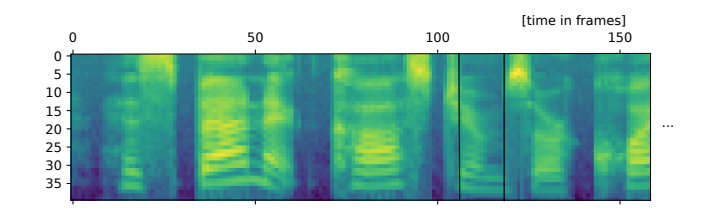
\includegraphics[width=0.9\textwidth]{speech_example}
  	\end{center}
\end{frame}

\begin{frame}
\frametitle{\#9 Your own idea here}
 \begin{itemize}
    \item As long as it is about text/speech
    \item And doable in a short time
   \end{itemize}
\end{frame}

\begin{frame}
\frametitle{Timeline}
 \begin{itemize}
    \item Find a project and a team (2 persons)
    \item Start small, reduce training data set size first!
     \item First use CPU, then if everything works, use GPUs
    \item Next week: Learn to use the Nvidia Tesla GPUs on the Hummel cluster (NVIDIA K80)
    \item We will have about one node (2 GPUs) per team
    \item Generate a public key: https://www.rrz.uni-hamburg.de/services/hpc/grundwissen/ssh-keys.html
   \end{itemize}
\end{frame}

\begin{frame}
\frametitle{Pretrained embeddings}
 \begin{itemize}
     \item In NLP tasks with little training data it may make sense to use precomputed embeddings:
     \item GoogleNews-vectors-negative300 - \url{https://code.google.com/archive/p/word2vec/}
     \item glove.840B.300d - \url{https://nlp.stanford.edu/projects/glove/}
     \item paragram\_300\_sl999 - \url{https://cogcomp.org/page/resource_view/106}
     \item wiki-news-300d-1M - \url{https://fasttext.cc/docs/en/english-vectors.html}
   \end{itemize}
\end{frame}

\begin{frame}[fragile]
\frametitle{Extra: Common voice}
  \begin{itemize}
	\item Recently released speech dataset from mozilla
	\item 20000 speakers, some information about age, gender and accent available
	\item Predict those attributes (separately or together)
  \end{itemize}
  \begin{Verbatim}[fontsize=\tiny]
  ['cv-valid-dev/sample-004039.mp3', 'are you enjoying london',
   '1', '0', 'thirties', 'female', 'england', '']
['cv-valid-dev/sample-004040.mp3', 'they placed the symbols of the pilgrimage on the doors of their houses',
 '3', '0', 'sixties', 'female', 'us', '']
['cv-valid-dev/sample-004041.mp3', 'he could always go back to being a shepherd',
 '3', '0', '', '', '', '']
['cv-valid-dev/sample-004042.mp3', 'its lower end was still embedded',
 '6', '0', 'twenties', 'female', '', '']
['cv-valid-dev/sample-004043.mp3', "i'm going into the desert the man answered turning back to his reading",
 '1', '0', '', '', '', '']
['cv-valid-dev/sample-004044.mp3', 'as the sun rose the men began to beat the boy',
 '2', '0', 'thirties', 'male', 'australia', '']
['cv-valid-dev/sample-004045.mp3', 'i have to find a man who knows that universal language',
 '3', '0', 'thirties', 'male', 'us', '']
['cv-valid-dev/sample-004046.mp3', 'the picnic was ruined by a marching band',
 '1', '0', 'twenties', 'male', 'scotland', '']
  \end{Verbatim}
\end{frame}

\begin{frame}[fragile]
\frametitle{Extra: One Million Posts Corpus}
  \begin{itemize}
\item DER STANDARD is an Austrian daily broadsheet newspaper. 
\item The data set contains a selection of user posts from the 12 month time span from 2015-06-01 to 2016-05-31. 
\item There are 11,773 labeled and 1,000,000 unlabeled posts in the data set.
\item Labels: \textbf{Sentiment} (negative/neutral/positive), \textbf{Off-Topic} (yes/no), \textbf{Inappropriate} (yes/no), \textbf{Discriminating} (yes/no)
  \end{itemize}
\end{frame}

% \end{frame}

%\section{Simple Optimization}
%
%% https://medium.com/@saxenarohan97/intro-to-tensorflow-solving-a-simple-regression-problem-e87b42fd4845
%% https://github.com/aymericdamien/TensorFlow-Examples/blob/master/examples/2_BasicModels/linear_regression.py
%\begin{frame}
%  \frametitle{Linear Regression}
%
%  \begin{itemize}
%  \item Given: $(x_1, y_1)$, \ldots, $(x_n,y_n)$
%  \item Goal: find $w$ and $b$ such that:
%    \begin{displaymath}
%      \argmin_{w, b} \frac{\sum^n_{i=1} (\hat{y}_i - y_i)^2}{n}
%    \end{displaymath}
%    where $\hat{y}_i = wx_i + b$.
%  \end{itemize}
%
%\end{frame}
%
%\begin{frame}[fragile]
%  \frametitle{Define model parameters}
%  Model: $\hat{y}_i = wx_i + b$
%
%\begin{lstlisting}
%w = tf.Variable(np.random.randn(), name="weight")
%b = tf.Variable(np.random.randn(), name="bias")
%\end{lstlisting}
%\end{frame}
%
%\begin{frame}[fragile]
%  \frametitle{Define the model}
%
%  \begin{displaymath}
%    \begin{pmatrix} \hat{y}_1\\\vdots\\\hat{y}_n\end{pmatrix} =
%    \begin{pmatrix} w\\\vdots\\w\end{pmatrix} *
%    \begin{pmatrix} \hat{x}_1\\\vdots\\\hat{x}_n\end{pmatrix} +
%    \begin{pmatrix} b\\\vdots\\b\end{pmatrix}
%  \end{displaymath}
%
%\begin{lstlisting}
%yhat = tf.add(tf.multiply(X, w), b)
%\end{lstlisting}
%
%{\footnotesize The scalars $w$ and $b$ are converted into vectors of the same
%  length as X (broadcast); \url{https://www.tensorflow.org/performance/xla/broadcasting}}
%
%\end{frame}
%
%\begin{frame}[fragile]
%  \frametitle{Define the loss}
%
%\begin{lstlisting}
%loss = tf.reduce_mean(tf.square(y - yhat))
%\end{lstlisting}
%
%\end{frame}
%
%
%\begin{frame}[fragile]
%  \frametitle{Optimization}
%
%\begin{lstlisting}
%epochs = 10
%optimizer = tf.train.GradientDescentOptimizer(
%    learning_rate).minimize(loss)
%
%with tf.Session() as sess:
%    ## initalize parameters
%    sess.run(tf.global_variables_initializer())
%
%    for i in list(range(epochs)):
%        ## run one epoch
%        sess.run(optimizer)
%        ## print result and loss
%        print(sess.run(yhat) + ' ' + sess.run(loss))
%\end{lstlisting}
%
%\end{frame}
%
%\begin{frame}[fragile]
%  \frametitle{Hands on: Simple optimization}
%
%  \begin{enumerate}
%  \item Do a linear regression to learn $y = 2x + 1$
%  \item Do a multiple linear regression with Boston housing prices
%  \end{enumerate}
%
%\begin{lstlisting}
%from sklearn.datasets import load_boston
%from sklearn.preprocessing import scale
%
%total_X, total_Y = load_boston(True)
%total_x = scale(total_x)
%\end{lstlisting}
%\end{frame}
%
%% https://www.tensorflow.org/tutorials/wide
%% https://github.com/aymericdamien/TensorFlow-Examples/blob/master/examples/2_BasicModels/logistic_regression.py
%\begin{frame}
%  \frametitle{Logistic regression}
%
%  TODO
%  tf.sigmoid
%
%\end{frame}
%
%\begin{frame}
%  \frametitle{Hands on: Regression model}
%
%  TODO: more complex example
%\end{frame}

\end{document}


%%% Local Variables:
%%% mode: latex
%%% TeX-engine: luatex
%%% End:
